\documentclass{AsignaturaResumen}

\def\ISMAIN{1}
\SetTitulo{Control de calidad}
\setabbreviationstyle[acronym]{long-short}
\makeglossaries

    % Glosario

\newglossaryentry{polimorfismo}{
    name={Polimorfismo},
    description={Existencia de dos o más variantes (alelos) de una secuencia de ADN en una población}
}
\newglossaryentry{locus}{
    name={Locus},description={Posición que ocupa un gen en el cromosoma}}
\newglossaryentry{amplicones}{
    name={Amplicones},
    description={Secuencias de ADN producidas por la amplificación de la hebra original en una \acrshort{pcr}. Se identifican como las bandas de una electroforesis en gel}
}
\newglossaryentry{sucesion microbiana}{
    name={Sucesión microbiana},
    description={Evento donde las especies de microorganismos presentes en una muestran son reemplazadas por otras}
}
\newglossaryentry{variante de secuencia}{
    name={Variante de Secuencia de Amplicón},
    description={Amplicón único de un conjunto de secuencias obtenidas en una secuenciación ya corregida}
}
\newglossaryentry{homopolimero}{
    name={Homopolímero},
    description={Secuencia repetitiva de nucleótidos (AGTGCGAT\emph{AAAA}TGCAGT, p.e.)}
}

    % Acrónimos

\newacronym{si}{SI}{Sistema Internacional}
\newacronym{iubmb}{IUBMB}{Unión Internacional de Bioquímica y Biología Molecular}

\newacronym{ros}{ROS}{especies reactivas de oxígeno}

\newacronym{pb}{pb}{pares de bases}
\newacronym{kb}{kb}{kilobases}

\newacronym{adn}{ADN}{Ácido desoxirribonucléico}
\newacronym{adnc}{ADNc}{ADN complementario}
\newacronym{dntps}{dNTPs}{desoxirribonucleótidos trifosfato}
\newacronym{ddntps}{ddNTPs}{didesoxinucleótidos}

\newacronym{adnpol}{ADNpol}{ADN polimerasa}

\newacronym{pcr}{PCR}{Reacción en Cadena de la Polimerasa}
\newacronym{rapd}{RAPD}{ADN Polimórfico Amplificado al Azar}
\newacronym{rflp}{RFLP}{Fragmentos de Restricción de Longitud Polimórfica}
\newacronym{dpcr}{dPCR}{PCR digital}
\newacronym{ngs}{NGS}{Secuenciación de Nueva Generación}
\newacronym{smrt}{SMRT}{Secuenciación en Tiempo Real de Molécula Única}

\newacronym{ccs}{CCS}{Lecturas de Consenso Circular}
\newacronym{asv}{ASV}{Variante de Secuencia de Amplicón}

\newacronym{iqi}{IQI}{Índice de Calidad Infaunal}

\newacronym{sds}{SDS}{dodecilsulfato sódico}
\newacronym{dms}{DMS}{dimetilsulfato}
\newacronym{ctab}{CTAB}{bromuro de cetiltrimetilamonio}

\begin{document}

    \frontmatter

\Portada
\Indices

    \mainmatter


\part{Fundamentos de control de calidad}
    
    \chapter{Introducción a la calidad} 
    \Quote{Trabajar en calidad significa diseñar, producir y servir un producto o servicio que sea útil, lo más económico posible y siempre satisfactorio para el usuario}{Kaoru Ishikawa}

    \resumebox{definicion}{Calidad}{Conjunto de valores y hábitos que, complementarios con el uso de prácticas y herramientas de calidad, permite el correcto cumplimiento de metas y objetivos}

\section{Costos de la calidad}

Hay varios tipos de costos relacionados a la calidad. Principalmente se pueden dividir en los costos por tener calidad y los costos por NO tener calidad.

En el caso de los primeros podemos encontrar costos por fallas tanto internas como externas. En el caso de las primeras podemos encontrar el reproceso de productos, el desperdicio de estos o los tiempos ociosos. En el caso de las segundas encontramos el costo de las devoluciones y reclamaciones de productos, el pago de garantías, así como las rebajas.

Por otro lado, los gastos por tener calidad están principalmente en la prevención y la evaluación. La prevención incluye cosas como la planeación de estrategias de caldidad, la capacitación del personal, la revisión de los productos y las auditorías (obtención y análisis de datos) La evaluación consisite en la verificación de los proveedores e inspecciones locales.
    \chapter{Filosofías de calidad} 

\begin{enumerate}
    \item Artesanal: Hacer las cosas bien a cualquier costo (material y de tiempo)
    \item Industrialización: Aumento en la producción pero de baja calidad
    \item Segunda guerra mundial: Determinación de la eficacia y de la entrega a tiempo como definición de calidad
    \item Posguerra: Alta cantidad de producción
    \item Control de calidad: Técnicas para insepccionar y evitar la salida de bienes defectuosos
    \item Aseguramiento de la calidad: Documentación de los procesos para asegurar el cumplimiento de las actividades de contro de calidad
    \item Gestión de calidad total: Visión que incluye al cliente en el cumplimiento de la calidad Es mucho más integral entre áreas, no como previo, enfocada en producción.
\end{enumerate}

\part{Herramientas estadísticas de calidad}

    \chapter{Histograma} 
\section{Histograma}




\section{Diagrama de Paretto}




\section{Diagrama de dispersión}




\section{Gráficas de control}



\subsection{Gráficas de control $X$}




\subsection{Gráficas de control $R$}




\section{Diagrama de Ishikawa}



    \chapter{Diagrama de Paretto} Este gráfico se basa en el principio de Pareto. Realizar un diagrama de Pareto ayuda a identificar estas "pocas causas" que, al resolverlas, se resuelven buena parte de los problemas.

    \resumebox{definicion}{Principio de Paretto}{Unas pocas causas son las que crean los mayores efectos.}

La realización de un diagrama de Paretto parte por la determinación de la situación general. Una vez conocido el problema general se determinan en qué categorías se catalogarán los problemas del proceso. Con esto listo se puede iniciar la recolección de datos alrededor de los problemas de un proceso y la asignación de cada uno de estos en una de las categorías determinadas.

Una vez se tienen los datos recolectados, lo primero a realizar es ordenarlos de mayor a menor. Posterior a esto, se calcula el porcentaje ($\%$, \autoref{eq:pareto_porcentaje}) que cada categoría representa de la cantidad de problemas total, así como el porcentaje acumulado ($\%_{Ac}$, \autoref{eq:pareto_porcentaje_acumulado}) de las categorías

\begin{equation}\label{eq:pareto_porcentaje}
    \% = 100\cdot\frac{x_{i}}{\sum{x_{i}}}
\end{equation}

\begin{equation}\label{eq:pareto_porcentaje_acumulado}
    \%_{Ac} = \sum{\%}
\end{equation}

Una vez se tienen todos estos datos, se elabora una gráfica con los datos ordenados de la siguiente manera

\begin{itemize}
    \item Eje X: Categorías de problemas
    \item Eje Y (Izquierda): Conteo de observaciones
    \item Eje Y (Derecha): Porcentaje acumulado
\end{itemize}

Con la gráfica lista, procedemos a trazar una linea en el punto en que se cruza el 80\% de porcentaje acumulado.

\begin{figure}\centering
    \resizebox{\linewidth}{!}{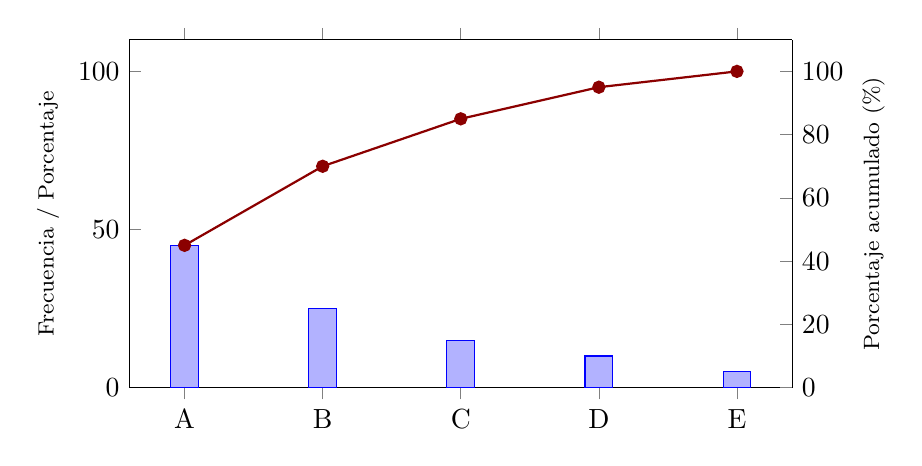
\begin{tikzpicture}
  \begin{axis}[
      width=10cm,height=6cm,
      ybar,ymin=0,ymax=110,
      axis y line*=left,
      ylabel={\footnotesize Frecuencia / Porcentaje},
      symbolic x coords={A, B, C, D, E},
      xtick=data
    ]
    \addplot coordinates {(A,45) (B,25) (C,15) (D,10) (E,5)};
  \end{axis}

  \begin{axis}[
      width=10cm,height=6cm,
      ymin=0,ymax=110,
      axis y line*=right,
      ytick={0,20,40,60,80,100},
      ylabel={\footnotesize Porcentaje acumulado (\%)},
      axis x line=none,
      symbolic x coords={A, B, C, D, E},
      xtick=data
    ]
    \addplot[DarkRed, thick, mark=*] coordinates {(A,45) (B,70) (C,85) (D,95) (E,100)};
  \end{axis}
\end{tikzpicture}}
    \rule{\linewidth}{0.5pt}
    \caption{Ejemplo de diagrama de Paretto}
    \label{fig:diagrama_de_pareto}
\end{figure}
    \chapter{Diagrama de dispersión} 
Este diagrama ayuda a encontrar si existe una relación entre variables y, de ser así, encontrar una expresión matemática que represente tal relación.

Esta relación puede ser:
\begin{itemize}
    \item Positiva: Una variable aumenta y la otra también
    \item Negativa: Una variable aumenta y la otra disminuye
\end{itemize}

En ambos casos la relación puede ser:

\begin{enumerate}
    \item Fuerte: Una variable aumenta/disminuye mucho y la otra también
    \item Debil: Una variable aumenta/disminuye mucho pero la otra aumenta/disminuye poco
\end{enumerate}

\begin{figure}\centering
    \resizebox{\linewidth}{!}{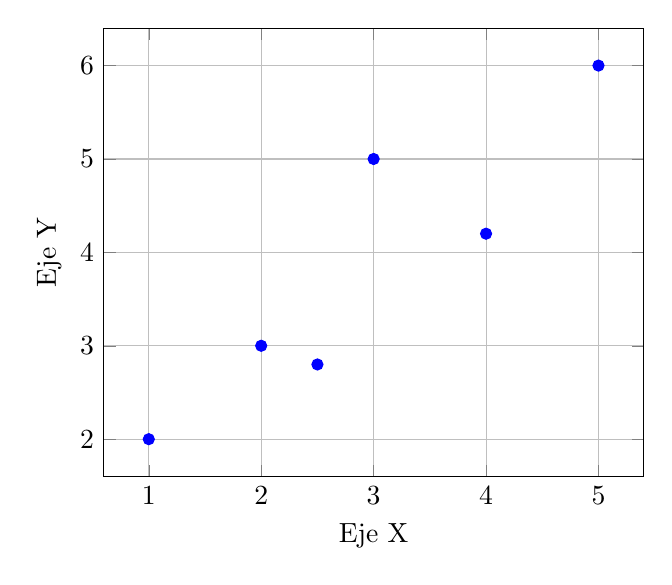
\begin{tikzpicture}
  \begin{axis}[
      xlabel={Eje X},
      ylabel={Eje Y},
      grid=major,
      only marks
    ]
    \addplot[blue, mark=*] coordinates {
      (1, 2) (2, 3) (2.5, 2.8) (3, 5) (4, 4.2) (5, 6)
    };
  \end{axis}
\end{tikzpicture}}
    \rule{\linewidth}{0.5pt}
    \caption{Ejemplo de diagrama de dispersión}
    \label{fig:diagrama_de_dispersion}
\end{figure}

\section{Obtención de modelo matemático}

Para poder obtener el modelo matemático que explique la relación entre variables nos apoyamos de la ecuación de la recta:

\begin{equation}
    y = a_{0} + a_{1}x
\end{equation}

Donde:

\begin{gather}
    a_{1} = \frac{n \sum{x_{i}y_{i}} - (\sum{x_{i}})(\sum{y_{i}}) }{ n \sum{x_{i}^{2}} - (\sum{x_{i}})^{2} }
    \\
    a_{0} = \bar{y} - a_{1}\bar{x}
\end{gather}

Despúes de esto es bueno evaluar cuan bien explica el modelo los datos, lo cual se hace con $r^{2}$ y $r$ ($\sqrt{r^{2}}$)

\begin{equation}
    r = \frac{n \cdot \sum{x_{i}y_{i}} - (\sum{x_{i}}\cdot\sum{y_{i}})}{\sqrt{n\sum{x_{i}^{2}} - (\sum{x_{i}})^{2}} \cdot \sqrt{n\sum{y_{i}^{2}} - (\sum{y_{i}})^{2}}}
\end{equation}

Donde el valor puede ir de -1 a 1, indicando el 0 un ajuste nulo, mientras que -1 y 1 significan un ajuste perfecto.

\section{Linearización}

Si bien mediante lo anterior se nos genera un modelo matemático que sigue una línea recta, cuando los datos están muy poco ajustados a esta linea la capacidad de predicción no es suficiente como para que sea un modelo válido. Para arreglar esto podemos identificar la forma en que se distribuyen los datos y manipularla para que se ajuste mejor a una línea recta, y así aumentar el coeficiente de correlación

Tenemos tres tipos principales de distribuciones:

\begin{itemize}
    \item Exponencial
    \begin{equation}
        y = \alpha \cdot e^{\beta x}
    \end{equation}

    \item Ley de potencias, o potencial
    \begin{equation}
        y = \alpha \cdot x^{\beta}
    \end{equation}

    \item Razón de crecimiento
    \begin{equation}
        y = \alpha \cdot \frac{x}{\beta + x}
    \end{equation}
\end{itemize}

\begin{figure}\centering
    \begin{subfigure}[b]{0.3\linewidth}
        \centering
        \resizebox{\linewidth}{!}{% 2. LEY DE POTENCIAS:  y = α · x^{β}
\begin{tikzpicture}
\begin{axis}[
    width=10cm, height=10cm,
    axis lines=left,
    xlabel={$x$}, ylabel={$y$},
    xtick=\empty, ytick=\empty,
    domain=0:5, samples=50,
    enlargelimits=false,
    legend pos=north west,legend style={draw=none}
]

\pgfmathsetmacro{\myalfa}{3}
\pgfmathsetmacro{\mybeta}{2}

\addplot[DarkRed, thick] {\myalfa*x^\mybeta};
\addlegendentry{\Large $y = \alpha \cdot x^{\beta}$}

\end{axis}
\end{tikzpicture}
}
        \rule{\linewidth}{0.5pt}
        \caption{Modelo potencial}
        \label{fig:modelo_potencial}
    \end{subfigure}
    \hfill
    \begin{subfigure}[b]{0.3\linewidth}\centering
        \resizebox{\linewidth}{!}{\begin{tikzpicture}
\begin{axis}[
    width=10cm, height=10cm,
    axis lines=left,
    xlabel={$x$}, ylabel={$y$},
    xtick=\empty, ytick=\empty,
    xmin=1.5, xmax=5,
    ymin=0, ymax=10,samples=100,
    enlargelimits=false,
    legend pos=north west,legend style={draw=none}
]

\addplot[DarkBlue, thick] {0.5*exp(0.6*x)};
\addlegendentry{\Large $y=\alpha e^{\beta x}$}

\end{axis}
\end{tikzpicture}}
        \rule{\linewidth}{0.5pt}
        \caption{Modelo exponencial}
        \label{fig:modelo_exponencial}
    \end{subfigure}
    \hfill
    \begin{subfigure}[b]{0.3\linewidth}\centering
        \resizebox{\linewidth}{!}{% 3. RAZÓN DE CRECIMIENTO:  y = α · x/(β + x)
\begin{tikzpicture}
\begin{axis}[
    width=10cm, height=10cm,
    axis lines=left,
    xlabel={$x$}, ylabel={$y$},
    xtick=\empty, ytick=\empty,
    domain=0:5, samples=50,
    enlargelimits=false,
    legend pos=south east,legend style={draw=none}
]

\pgfmathsetmacro{\myalfa}{3}
\pgfmathsetmacro{\mybeta}{2}

\addplot[Green, thick] {\myalfa*x/(\mybeta+x)};
\addlegendentry{\Large $y = \alpha \cdot \frac{x}{\beta+x}$}

\end{axis}
\end{tikzpicture}}
        \rule{\linewidth}{0.5pt}
        \caption{Modelo de razon de crecimiento}
        \label{fig:modelo_razon_de_crecimiento}
    \end{subfigure}
    
    \rule{\linewidth}{0.5pt}
    \caption{Ejemplo de cada uno de los modelos}
    \label{fig:modelos}
\end{figure}

Para resolver cada tipo de distribución nos ayudamos de las propiedades de los logaritmos.

\begin{gather}
    \log(a \cdot b) = \log(a) + \log(b)
    \\
    \log \left(\frac{a}{b}\right) = \log(a) - \log(b)
    \\
    \log(a^{b}) = b \cdot \log(a)
    \\
    \log(\sqrt[b]{a}) = \frac{\log(a)}{b}
\end{gather}

\subsection{Exponencial}

\begin{gather}
    \ln(y) = \ln(\alpha \cdot e^{\beta \cdot x})
    \\
    \ln(y) = \ln(\alpha) + \ln(e^{\beta \cdot x})
    \\
    \ln(y) = \ln(\alpha) + \beta \cdot x
    \\
    \hline
    \\
    x = x \quad;\quad y = \ln(y)
    \\
    a_{0} = \ln(\alpha) \quad;\quad a_{1} = \beta
\end{gather}

\subsection{Ley de potencias, o potencial}

\begin{gather}
    \log(y) = \log(\alpha \cdot x^{\beta})
    \\
    \log(y) = \log(\alpha) + \log(x^{\beta})
    \\
    \log(y) = \log(\alpha) + \beta \cdot \log(x)
    \\
    \hline
    \\
    x = \log(x) \quad;\quad y = \log(y)
    \\
    a_{0} = \log(\alpha) \quad;\quad a_{1} = \beta
\end{gather}

\subsection{Razón de crecimiento}

\begin{gather}
    (y)^{-1} = \left(\alpha \cdot \frac{x}{\beta + x}\right)^{-1}
    \\
    \frac{1}{y} = \frac{\beta + x}{\alpha \cdot x}
    \\
    \frac{1}{y} = \frac{\beta \cdot 1}{\alpha \cdot x} + \frac{x}{\alpha \cdot x}
    \\
    \frac{1}{y} = \frac{\beta}{\alpha} \cdot \frac{1}{x} + \frac{1}{\alpha}
    \\
    \hline
    \\
    x = \frac{1}{x} \quad;\quad y = \frac{1}{y}
    \\
    a_{0} = \frac{1}{\alpha} \quad;\quad a_{1} = \frac{\beta}{\alpha}
\end{gather}
    \chapter{Gráficas e índices de control} 

\section{Gráficas de control $X$}




\section{Gráficas de control $R$}




\section{Índices de capacidad de procesos}

\subsection{$C_{p}$}

El $C_{p}$ mide la capacidad potencial de un proceso

\begin{equation}
    C_{p} = \frac{\mathrm{ES} - \mathrm{EI}}{6\sigma}
\end{equation}

Donde:

\begin{itemize}
    \item $\mathrm{ES}$ es el límite superior
    \item $\mathrm{EI}$ es el límite inferior
    \item $\sigma$ es la desviación estandar
\end{itemize}

\subsubsection{$C_{pi}$ y $C_{ps}$}

Es posible calcular asímismo la capacida unicamente inferior ($C_{pi}$) o unicamente superior ($C_{ps}$). La forma de calcular ambos deriva de la fórmula de $C_{p}$, solo que tomando en cuenta solo un lado de la campana de distribución de datos

En el caso del $C_{pi}$ este corresponde al limite inferior del cual el proceso no debe de bajar

\begin{equation}
    C_{pi} = \frac{\mu-\mathrm{EI}}{3\sigma}
\end{equation}

Por otro lado, el $C_{ps}$ indica el limite superior el cual el proceso no debe superar

\begin{equation}
    C_{ps} = \frac{\mathrm{ES}-\mu}{3\sigma}
\end{equation}

\subsection{$C_{pk}$}

El $C_{pk}$ es un indicador de la capacidad de un proceso de generar productos con las características deseadas de manera exitosa.

Su cálculo se realiza de la siguiente manera:

\begin{equation}
    C_{pk} = \mathrm{Min}\left[\frac{\mathrm{ES}-\mu}{3\sigma},\frac{\mu-\mathrm{EI}}{3\sigma}\right]
\end{equation}

\subsubsection{Índice $k$}

Para el índice de $C_{pk}$ se puede calcular también el valor de $k$, el cual nos indica cuan centrado está un proceso:

\begin{equation}
    k = \frac{\lvert\ \mu-N \ \rvert}{\frac{1}{2} \cdot (\mathrm{ES - EI})} \cdot 100
\end{equation}

\subsection{$C_{pm}$}

Similar al $C_{pk}$, pero este además toma en cuenta también cuán centrados están los datos y la variabilidad de estos de forma simultanea.

\begin{equation}
    C_{pm} = \frac{\mathrm{ES}-\mathrm{EI}}{6\tau}
\end{equation}


Donde $\tau$ representa la variabilidad del proceso respecto al valor nominal ($N$), y se calcula de la siguiente manera:

\begin{equation}
    \tau = \sqrt{\sigma^{2} + (\mu - N)^{2}}
\end{equation}


El valor nominal ($N$) representa el valor que se busca alcanzar en el proceso

\subsection{Interpretación de índices}

Los valores obtenidos en los índices anteriores se pueden interpretar de la siguiente manera:

\begin{align}
    <1 &= \text{Proceso no capaz}
    \\
    1 &= \text{Cumple justo}
    \\
    1.33 &= \text{Proceso capaz}
    \\
    1.67 &= \text{Proceso muy capaz}
    \\
    >2 &= \text{Excelente capacidad}
\end{align}
    \chapter{Diagrama de Ishikawa o Causa-Efecto} \input{07}

%\part{Herramientas administrativas de calidad}
%
%   \chapter{}
%
%\part{Sistemas de gestión de calidad}
%
%    \chapter{Norma ISO 9001}
%    \chapter{Norma ISO 14001}
%    \chapter{Riesgos y oportunidades de un SGC}
%
%\part{Metodología Seis Sigma}
%
%    \chapter{Introducción a metodología Seis Sigma}
%    \chapter{Modelo DMAIC}


    \PlainGeom
    \appendix



    \backmatter

\Bibliografia
\Glosarios

\end{document}